\documentclass{article}
\usepackage{graphicx}
\usepackage{makecell}
\usepackage{listings}
\usepackage{color}
\usepackage{apacite}%Also use in Capstone
\usepackage[utf8]{inputenc}
\usepackage[letterpaper, margin=1.25in]{geometry}
\pagenumbering{arabic}
\title{IB Computer Science IA | Attendance System for the Marching Band}
\author{Jacob Samurin}

\definecolor{dkgreen}{rgb}{0,0.6,0}
\definecolor{gray}{rgb}{0.5,0.5,0.5}
\definecolor{mauve}{rgb}{0.58,0,0.82}

\lstset{frame=tb,
	language=Java,
	aboveskip=3mm,
	belowskip=3mm,
	showstringspaces=false,
	columns=flexible,
	basicstyle={\small\ttfamily},
	numbers=left,
	numberstyle=\tiny\color{gray},
	keywordstyle=\color{blue},
	commentstyle=\color{dkgreen},
	stringstyle=\color{mauve},
	breaklines=true,
	breakatwhitespace=true,
	tabsize=3
}

\begin{document}
%TODO Comment this out when turn in
\maketitle
\newpage
\tableofcontents
\newpage
%To here
\section{Criterion A: Planning}
\subsection{Defining the Problem}
The problem of Mr. Todd Fessler (my client) is that for our marching band class there is no good and efficient way of taking attendance. The way of taking attendance right now is that the “Drum Majors” who are the overall leaders in the marching band, go around and ask each row for their attendance, and it took a very long time to take attendance.
\subsection{Rational for Proposed Solution}
My solution will make it possible for the leaders of each row to take attendance then the Drum Majors won’t have to go row by row. This will also skip the Drum Major step completely since my client will have direct accesses to the app. This will make it easier for everyone and faster, so we can have a longer rehearsal times.
\subsection{Success Criterion}
\begin{center}
	\begin{tabular}{|l|}
		\hline
		Different classes each level of leaders\\
		\hline
		A web app will be created add the different levels can edit different kinds of pages\\
		\hline
		Make it accessible from a phone\\
		\hline
		Make it accessible from an iPad\\
		\hline
		Make it accessible from a laptop/computer\\
		\hline
		Have the sever running the web app set up\\
		\hline
	\end{tabular}
\end{center}
\newpage
\section{Criterion B: Solution Overview}
\subsection{Sketch}
\subsection{UML Diagram}
This is the basic outline of the different classes and data types \\ \\
%TODO Update ASAP
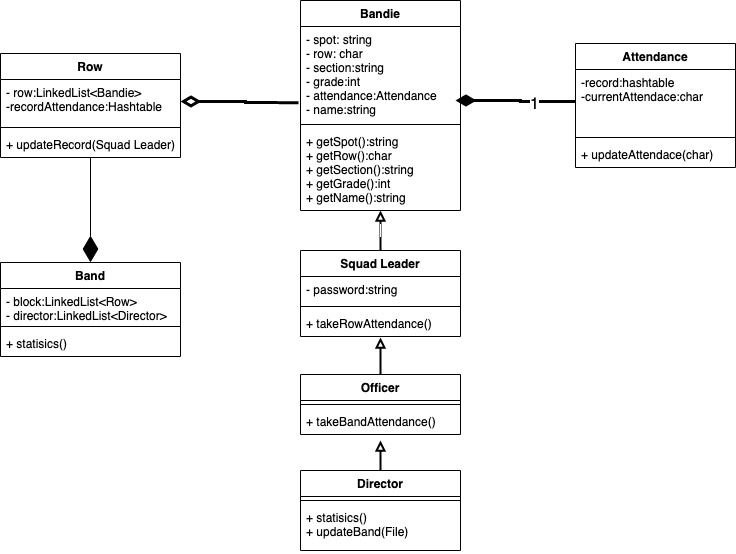
\includegraphics[width=6in]{IA UML and Flowchart-UML.jpg}
\subsection{Flowchart}
This is the basic flow of the \verb|updateBand| method \\ \\
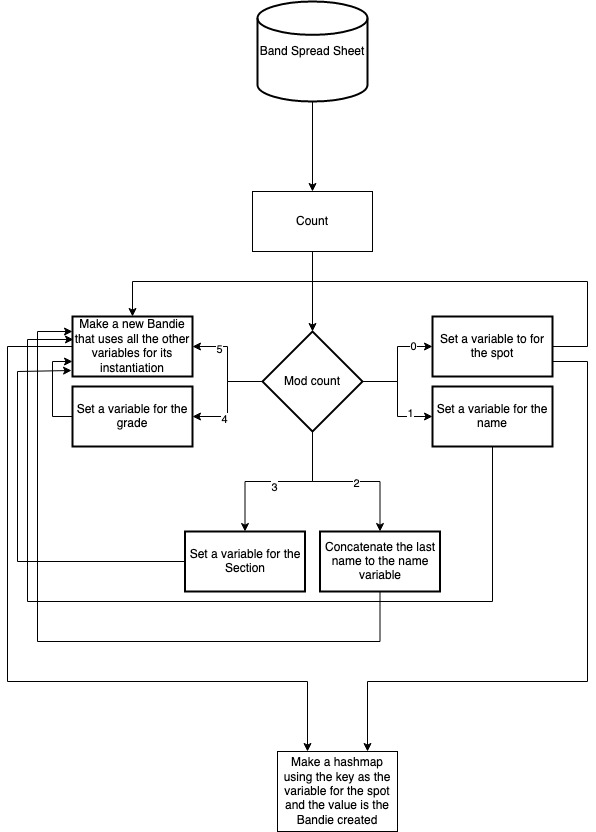
\includegraphics[width=6in]{IA UML and Flowchart-Flowchart.jpg}
\subsection{Pseudocode}
For the pseudocode I will be writing out the \verb|updateBand| method
\begin{verbatim}
				item = read in a file for every section that stops in a comma
				while there is a next item
					if tem%6 equals 0 
						spot = item
						if its k-row
							row = first 2 letter
						else
							row = first letter
					if temp%6 equals 1
						name = item + " "
					if temp%6 equals 2
						name += item
					if temp%6 equals 3
						section = item
					if temp%6 equals 4
						grade = item
					if temp%6 equals 5
						new object t of type Top(spot, row, name, section, grade, item)
					temp++
\end{verbatim}
\subsection{Development Plan}
This is a plan for how to create the final product
\begin{itemize}
	\item Create the \verb|Bandie| class and the other levels of authorization all the way to Director/Admin
	\item Write the Row class with the hash table for the whole row’s attendance and a linked list for the Bandies in the Row
	\item Create the Band class with the linked list for the directors and another linked list for the rows
	\item Create the Attendance class to store the past and current attendance for each \verb|Bandie|
	\item Be able to upload a new CSV file to upload the structure of the band
	\item Store past attendance for each \verb|Bandie| in a CSV file
	\item Make a web app that will ...
		\begin{enumerate}
			\item Have a login screen where any level above \verb|Bandie| has a password
			\item Have the different screens for Bandies, Squad Leaders, and Drum Majors.
			\item For Directors, they will also have a Statistics page with a tagline at the top(refer to the Sketch above)
		\end{enumerate}
\end{itemize}
\subsection{Test Cases}
\resizebox{6in}{!}{
	\begin{tabular}{|p{3in}|p{3in}|}
		\hline
		\LARGE Case & \LARGE Outcome\\
		\hline \hline \\
		\Large Logging into a higher level account &
		\begin{itemize}
			\item An incorrect password will send errors to the user.
			\item A correct password will let the user through.
			\item An invalid password(i.e. sending in the wrong data type) will send an error to the user 
		\end{itemize}
		\\
		\hline \\
		\Large Uploading a spreed sheet file &
		\begin{itemize}
			\item If the file is not a CSV file then will pass an error to the user "Improper File type"
			\item If the file is a CSV but is not properly formatted it will pass an error to the user "Improper formatted"
			\item If the file is a CSV and the first line is properly formatted it will upload the file
		\end{itemize}
		\\
		\hline %\\
		% \Large Input for the attendace &
		% \begin{itemize}
		% 	\item
		% \end{itemize}
		% \\
		% \hline
	\end{tabular}
}
\subsection{Record of Tasks}
\resizebox{6in}{!}{
	\begin{tabular}{| c | p{1.5in} | p{1.5in} | p{1in} | p{1in} | c |}
		\hline
		Task Number & Planned Action & Planned Outcome & Time Estimated (Minutes) & Target Completion Date & Criterion\\
		\hline
		1 & Brainstorming with my client & An idea for the project & 30 & May 5, 2022 & A\\
		\hline
		2 & Interview & Get to know what my client wants & 8.5 & May 24, 2022 & A\\
		\hline
		3 & Write a draft proposal & proposed to teacher & 60 & May 26, 2022 & A\\
		\hline
		4 & Write a proposal & Re-proposed  to teacher & 75 & Aug 22, 2022 & A\\
		\hline
		5 & make a Record of Tasks & Organize a timeline & 15 & Aug 23, 2022 & B\\
		\hline
		6 & Second Interview & Get a better Idea from my client & 7 & Sep 1, 2022 & A\\
		\hline
		7 & Create UML diagram & Get a UML diagram & 90 & Oct 20, 2022 & B\\
		\hline
		8 & Working on criterion B & Complete the outline of the criterion B & 20 & Oct 21, 2022 & B\\
		\hline
		9 & Third Interview  & Get a better idea of the statistics section & 6 & Oct 26, 2022 & A\\
		\hline
		10 & Create drawing UI & To put my idea on to paper & 45 & Nov 5, 2022 & B\\
		\hline
		11 & Re-setup the document & Make it easier to work on the document & 180 & Nov 8, 2022 & A/B\\
		\hline
		12 & added a case to the Test Cases section & Work on a part needed for the finishing Criterion B& 45 & Nov 9, 2022 & B\\
		\hline
		13 & added a case to the test case's section & work on a part needed for the finishing criterion b& 15 & Nov 9, 2022 & B\\
		\hline
		14 & Fix the UML and finish Flowchart and Pseudocode & fixed UML and finished Flowchart and Pseudocode & 90 & Dec 19, 2022 & B\\
		\hline
		15 & writing the hash table section & started work on the writing part of criterion C & 30 & Jan 8, 2023 & C\\
		\hline
		16 & Coding to complete criterion c & complete the coding for criterion c & 240 & Feb 4, 2023 & C\\
		\hline
	\end{tabular}
}
\newpage
\section{Criterion C: Development}
\subsection{Program Structure}
The main parts of my program are the \verb|App.java|, \verb|Bandie.class|, \verb|Row.java|, and \verb|Band.java|. The \verb|App| class, this has my main method and the details for my basic Terminal User Interface(TUI). The \verb|Bandie| class is used as a base for my inheritance for every member of the band. \verb|Row.java| is using a LinkedList\cite{linkedList} of \verb|Bandie| to simulate what row would look link in real life. The final class \verb|Band| is working like a HashTable\cite{hashTable} because it contains a LinkedList\cite{linkedList} of \verb|Row|. This make \verb|Band.java| act like a band block would even have a dynamic amount of people on each row by using the \verb|Row| object.\\
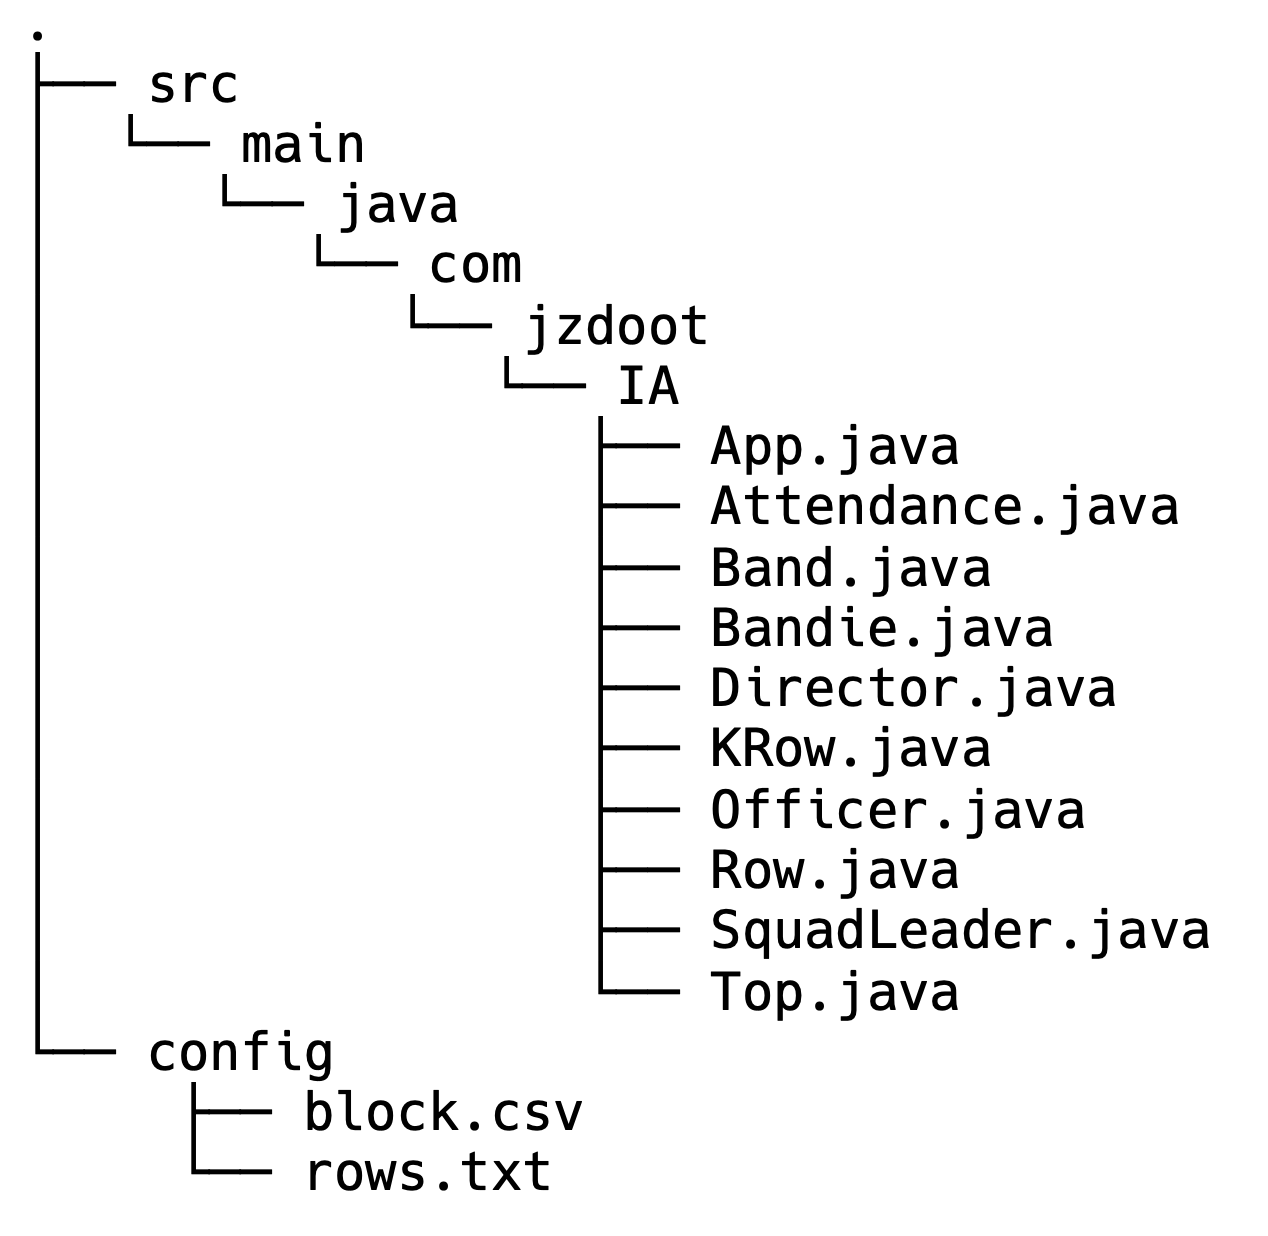
\includegraphics[width=3in]{fileStructure.png}
\subsection{Techniques Used}
\begin{itemize}
	\item Inheritance
	\item Polymorphism
	\item Encapsulation
	\item File Reading and Writing
	\item HashTable\cite{hashTable}
	\item LinkedList\cite{linkedList}
	\item HashMaps\cite{hashMap}
	\item Singleton Class
\end{itemize}
\subsubsection{Inheritance}
I'm using inheritance as a way to easily have the same base for all my users. Each user (except Directors) are inheriting aspects from \verb|Bandie| and other objects. The major point of using this was to make is easy to instantiate any of the users in my program. Here is an example from my \verb|Director| class.
\begin{lstlisting}
// Director.java
		Bandie current = new Bandie(); // This is setting up a default
		Director direct  = new Director();
		LinkedList<Row> newBlc = new LinkedList<Row>();
		boolean dir = false;
		Scanner s = new Scanner(f);
		String name = "";
		s.useDelimiter(",");
		int count=0,realCount=0;
		if(topLine)
			s.nextLine();
		while(s.hasNext()){
			String item = s.next();
			switch(count%6){
				case 0:
					switch(item){ //Here is were we actualy where we can make this a any other type of user
						case "director":
							dir=true;
							break;
						case "officer":
							current = new Officer(); //This will change current into an Officer
							break;
						case "leader":
							current = new SquadLeader();//This will change current into an Squad Leader
							break;
						case "bandie":
							current= new Bandie();//This will keep current the same as the default of Bandie
							break;
					}
					break;
\end{lstlisting}
On line 2 we set a default and the left-hand side of the instantiate, down at line 16 we have a switch case which well make the \verb|current| on line 2 into any other type of user from lines 21 to 27. 
\subsubsection{Polymorphism}
Polymorphism is when you have different classes that know what they are and what they can do. I'm using this when I'm calling the \verb|takeAttendance| and the \verb|takeRowAttendance| between when \verb|Director|, \verb|Officer|, or \verb|SquadLeader| call it.
\begin{lstlisting}
//SquadLeader.java
public void takeRowAttendance(char[] a){
	Band.getRow(super.getRow()).updateRecord(this);
	for (int i = 0; i < Band.getRow(super.getRow()).size(); i++) {
		takeAttendance((""+super.getRow())+(i+1), a[i]);
	}
}
public void takeAttendance(String spott, char a
	Band.getBandie(spott).setAttendance(a);
}

//Office.java
public void takeRowAttendance(char row, char[] a){
	Band.getRow(row).updateRecord(this);
	for (int i = 0; i < Band.getRow(row).size(); i++) {
		super.takeAttendance((""+row)+(i+1), a[i]);
	}
}

//Director.java
public void takeRowAttendance(char row, char[] a){
	Band.getRow(row).updateRecord(this);
	for (int i = 0; i < Band.getRow(row).size(); i++) {
		takeAttendance((""+row)+(i+1), a[i]);
	}
}
public void takeAttendance(String spott, char a){
	Band.getBandie(spott).setAttendance(a);
}
\end{lstlisting}
This example is showing the difference between the \verb|takeRowAttendance| method in \verb|SquadLeader| on line 1 and \verb|Offcer|/\verb|Director| on line 12 and 20. The \verb|takeRowAttendance| on line 2 us more so used when the row is predefined like in \verb|SquadLeader.java| where they can only change their row. But the \verb|takeRowAttendance| on line 13 and 21 can change any row that is asked.
\subsubsection{Encapsulation}
Encapsulation is the practice of keeping everything contained in one object and using accessor methods to get values. I use this in the \verb|Row| class because I don't have access to the LinkedList\cite{linkedList} it's self, but I can get the size trough the \verb|size()| method. Here is that example
\begin{lstlisting}
//Attendance.java
package com.jzdoot.IA;
import java.util.Date;
import java.util.HashMap;

public class Attendance{
	private HashMap<Date,Character> record;
	//NOTE the currentAttendace is now in the bandie class

	public void updateAttendance(char attendance){
		record.put(new Date(), attendance);
	}
}
\end{lstlisting}
In this example the HashMap\cite{hashMap} on line 7 is private and the method \verb|updateAttendance| on line 10 is used to set the HashMap\cite{hashMap} instead of changing the HashMap\cite{hashMap} directly.
\subsubsection{File Reading and Writing}
File reading and writing is a way for a program to read in a file and output out to a file. I'm using it in one main way, in the \verb|Director| class there is a method called \verb|updateBand| it is used to update the block structure easily by using a \verb|.csv| file because it's stored in plain text but can be edited by any spreadsheet software. I use this to store the band and to reset it when the program gets closed. To store this copy this file to a new file in a saved directory\cite{moveFile}.
\subsubsection{HashTable}
HashTables\cite{hashTable} are arrays of LinkedLists\cite{linkedList}. I'm using this differently I made a LinkedList\cite{linkedList} of \verb|Row|, but \verb|Row| is a LinkedList\cite{linkedList} of \verb|Bandie| this works in the same general way as a HashTable\cite{hashTable}. The way I'm using this "HashTable" is to store the structure of the band and each row will be able to be dynamic and so will the number of rows which is why I didn't use just a normal HashTable\cite{hashTable}.
\subsubsection{LinkedList}
A LinkedList\cite{linkedList} is a list where each item is a linked node which have two values. One of the values is the value you give the item. The other is a link to the next item. I use this throughout my project in almost every class. Here are some examples:
\begin{lstlisting}
//Band.java
private static LinkedList<Row> block;
public static void init() throws FileNotFoundException{
	if(instance != null)
		System.out.println("Error: instance already exists");
	else{
		instance = new Band();
		int kCount = 0;
		Scanner s = new Scanner(new File("config/rows.txt"));
		while(s.hasNext()){
			String item = s.nextLine();
			char r = item.charAt(0);
			//TODO add exception for krow
			if(r != 'k')
				addRow(new Row(r));
			else{
				kCount++;
			}
		}
		LinkedList<LinkedList<Bandie>> kr = new LinkedList<LinkedList<Bandie>>();
		for(int i=0;i<=kCount;i++)
			kr.add(new LinkedList<Bandie>());
		addRow(new KRow(kr));
	}
}
public static void addRow(Row r){
		if(block.size() > 0)
			for(int i=0; i<block.size();i+=0){
				if(block.get(i).compareTo(r)<0)
					i++;
				else if(block.get(i).compareTo(r)==0){
					System.out.println("already exists");
					break;
				}else if(block.get(i).compareTo(r)>0){
					block.add(i, r);
					break;
				}else
					block.add(r);
			}
		else
			block.add(r);
}
public static Row getRow(char row){
	for(Row arr : block){
		if(arr.getLetter()==row)
			return arr;
	}
	return null;
}
\end{lstlisting}
Here we use a LinkedList\cite{linkedList} to store the band block, and we write the left-hand side of the instantiate of the LinkedList on line 2. I put in two other methods in that use this LinkedList \verb|init| and \verb|addRow|. This benefits from using a LinkedList instead of a ArrayList\cite{arrayList} because the LinkedLists are better at iterate and getting items out. ArrayList are better for just storing items.
\subsubsection{HashMaps}
HashMaps\cite{hashMap} are a set of "keys" and "values". Keys can't repeat but values can. you can use the keys to accesses the values. I use HashMaps in the \verb|Attendance| and \verb|Row| classes. Here is an example:
\begin{lstlisting}
//Attendance.java
private HashMap<Date,Character> record;
public Attendance(){
	record=new HashMap<Date,Character>();
}
public void updateAttendance(char attendance){
	record.put(new Date(), attendance);
}
//Row.java
private Map<Date, Top> recordAttendance;
public void updateRecord(Top sl){
	recordAttendance.put(new Date(), sl);
}
\end{lstlisting}
We start the instatation on line 2 and call it \verb|record|. We update \verb|record| on line 7. We use the HashMap on line 10 the same way it is just the best way to store this kind of data.
\subsubsection{Singleton Class}
A Singleton Class is a style of writing a class that makes sure there is only one instance of the object. I use this style of writing a class in my \verb|Band| class. The most important part is the \verb|init()| method I wrote. This method will start by making sure there is an instance of \verb|Band| and creating all the rows for the block. The usefulness of the Singleton Class structure here is that I can call that same \verb|Band| instance from anywhere in the program. This makes it much easier to modify this object in all scenarios.
\newpage
\section{Criterion E: Evaluation}
\newpage
\section{Appendix A: Interview}
Interview conducted in person
Interview 1 initial information gathering

Student - Basically my plan right now for the for the program is there's going to be different tiers. So, there’s going to be a squad leader tier, a drum major tier, and then a director/admin tier. Squad leaders will be able to change attendance within the row, for Drum Major will be able to change attendance for the entire band and then for directors they can change the attendance for the entire band and on top of that there's some statistics like what rows haven't taken attendance yet, who turned into attendance for which row, and then maybe some row of the week stuff like most improved week to week, move most improved within the week, or best overall within the week or for the entire year. I’ll be able to collect all that kind of data just from attendance.
Client – That’s awesome. So would it be like you're thinking, like you said squad leaders have control over their rows. 
Student - and then drum majors the entire band and then you guys can take this for the entire band and then you guys can do attendance for the entire band and then on top of that you can look at statistics and stuff
Client - Is there any way once like for example of this squad leaders have submitted their attendance for the day is there a way for them to update it?
Student - I mean I could definitely implement that.
Client - or like a way for them to update it until the end of class. Somebody shows up that's the issue I think yeah if somebody shows up late on excused then they're marked absent for the whole day, but we need to know if they were late that day or if they were asking because that changes 
Student –I can probably set up a window of time like every morning from like 7:30 to 8:30 maybe even earlier I can set it to like 7 like to whenever time the period ends nowadays. Talking about some basic structure %2:04
\newpage
\section{Appendix B: References}
\bibliography{IA}{}
\bibliographystyle{apacite}
\end{document}
